\documentclass[12pt,letterpaper]{article}

\usepackage[spanish,es-tabla]{babel}
\usepackage[utf8]{inputenc}
\usepackage[T1]{fontenc}
\usepackage{geometry}
\usepackage{setspace}
\usepackage{graphicx}
\usepackage{booktabs}
\usepackage{hyperref}
\usepackage{amsmath}
\usepackage{amssymb}
\usepackage{adjustbox}
\usepackage{float}
\usepackage{cite}

\geometry{margin=2.5cm}
\setstretch{1.15}

\hypersetup{
    colorlinks=true,
    linkcolor=black,
    urlcolor=blue,
    citecolor=blue
}

\title{\textbf{Proyecto Integrador de Machine Learning II}\\
\large Tercera Entrega (Final): Modelamiento Econométrico Avanzado, Ensambles de Aprendizaje Automático, Contraste Metodológico y Despliegue en Producción}

\author{
    Julian Duarte \\
    Julian Jimenez
} 

\date{Asignatura: Machine Learning II\\
Docente: Wilmer Pineda-Ríos\\
Universidad Externado de Colombia\\
Noviembre de 2026}

\begin{document}

\maketitle

\begin{abstract}
Este documento constituye el informe técnico de la Tercera Entrega (Final) del proyecto integrador. Se aborda la predicción del precio y rentabilidad de criptomonedas (BTC, ETH, DOGE) expresadas en pesos colombianos (COP), adaptando y contrastando rigurosamente el trabajo de Gautam (2025). Ante las observaciones docentes sobre la aparente dominancia de la línea base en niveles de precios, se fundamenta teórica y econométricamente la no estacionariedad de las series mediante contrastes de raíz unitaria (ADF y KPSS), justificando formalmente la diferenciación hacia retornos e ilustrando el fenómeno mediante análisis de autocorrelación (ACF/PACF). Se formula y optimiza una batería completa de modelos de series de tiempo complejas: SARIMAX con variables exógenas (TRM oficial de Colombia, RSI, MACD), heterocedasticidad condicional mediante GARCH(1,1) con innovaciones Student's $t$, y dinámicas multivariadas a través de modelos VAR y de Corrección de Errores Vectoriales (VECM) fundamentados en el test de cointegración de Johansen. Dichas aproximaciones se contrastan frente a los ensambles avanzados del curso (XGBoost, LightGBM, CatBoost y Random Forest) y contra los resultados empíricos del artículo base. Finalmente, se documenta la arquitectura del aplicativo web interactivo desplegado en Vercel para la toma de decisiones financieras en tiempo real.
\end{abstract}

\tableofcontents
\newpage

\section{Introducción y Justificación Metodológica de la Entrega Final}

El presente informe consolida la \textbf{Fase 3: Consolidación, despliegue y comunicación de resultados} del Proyecto Integrador. El objetivo central consiste en construir un sistema predictivo robusto, interpretable y desplegado en producción web para el pronóstico del valor de activos criptográficos en pesos colombianos (COP).

A partir de la retroalimentación docente de la segunda entrega, este documento profundiza directamente en la estructura generadora de datos y en la formulación rigurosa de los modelos predictivos, prescindiendo de discusiones accesorias. Se resuelven con rigor econométrico tres interrogantes medulares:
\begin{enumerate}
    \item \textbf{Causa de la dominancia de la persistencia ingenua en niveles:} Se demuestra analítica y empíricamente que a frecuencia horaria, una serie integrada de orden uno $I(1)$ induce un error cuadrático y porcentual artificialmente bajo para la persistencia ($y_{t+1} \approx y_t$), fenómeno derivado de la caminata aleatoria.
    \item \textbf{Necesidad de la diferenciación y modelado de retornos:} Se justifica por qué la transformación a retornos relativos $\Delta \ln P_t \approx \frac{P_t - P_{t-1}}{P_{t-1}}$ restablece la estacionariedad $I(0)$, permitiendo que los modelos avanzados capturen auténtica capacidad predictiva sobre la dirección del mercado (\textit{Directional Accuracy / Hit Ratio}).
    \item \textbf{Ampliación del espacio de modelos:} Se introducen y optimizan modelos econométricos sofisticados (SARIMAX con exógenas, GARCH con distribuciones pesadas, VAR y VECM cointegrado), contrastándolos de manera transparente con los ensambles tabulares avanzados propuestos por Gautam (2025).
\end{enumerate}

\section{Fundamentación Econométrica: Raíces Unitarias, Diferenciación y Cointegración}

\subsection{Evolución Histórica y Canal Cambiario TRM}
La dinámica del valor de un criptoactivo en Colombia está expuesta a un doble riesgo de mercado: la volatilidad inherente al activo criptográfico y la fluctuación cambiaria del peso colombiano (COP) frente al dólar estadounidense (USD). La Figura~\ref{fig:price_trm} ilustra la serie histórica horaria analizada (febrero a octubre de 2026), evidenciando episodios de correlación y desacople entre la TRM y el precio del activo.

\begin{figure}[H]
\centering
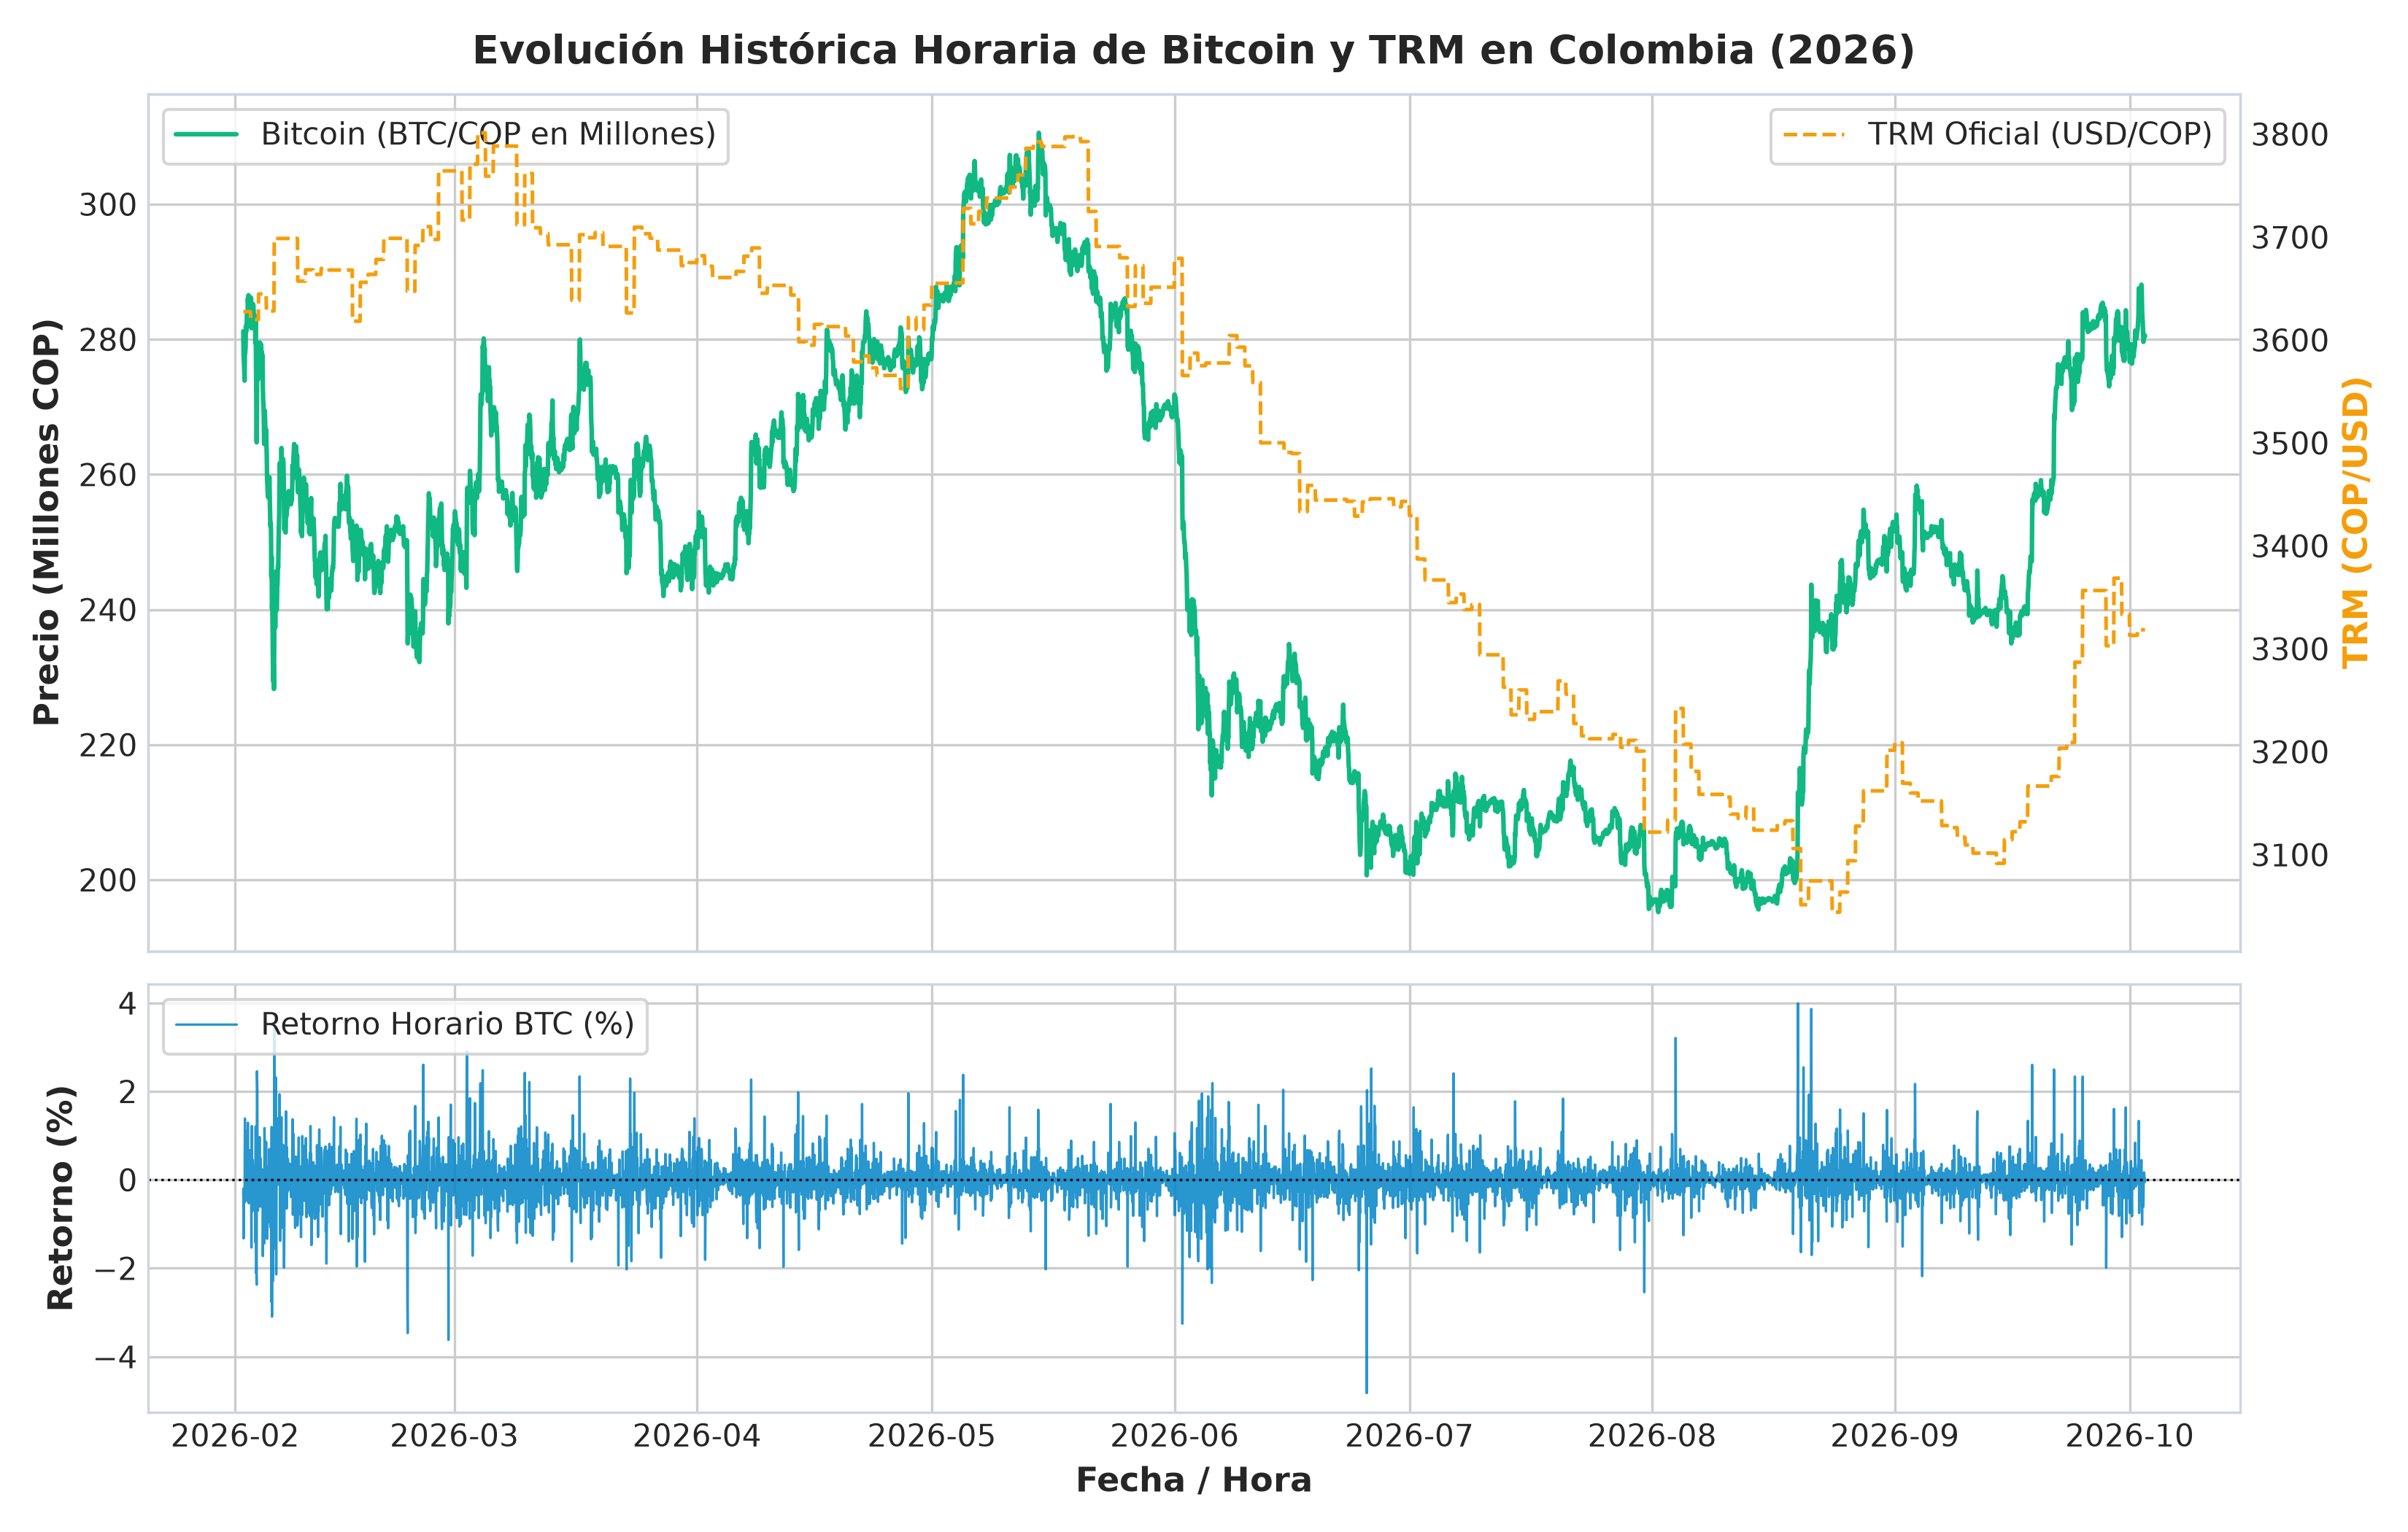
\includegraphics[width=0.92\textwidth]{figures/fig1_price_trm_returns.png}
\caption{Evolución temporal horaria de Bitcoin en COP (eje izquierdo), Tasa Representativa del Mercado (eje derecho) y retornos porcentuales horarios diferenciados.}
\label{fig:price_trm}
\end{figure}

\subsection{Contrastes de Estacionariedad: ADF y KPSS}
Para determinar formalmente el orden de integración de las series de precios horarios en COP ($P_t^{\text{COP}} = P_t^{\text{USD}} \times \text{TRM}_t$) y de la TRM, se aplicaron dos contrastes complementarios sobre el conjunto de entrenamiento (garantizando ausencia de fuga de información):
\begin{itemize}
    \item \textbf{Test Aumentado de Dickey-Fuller (ADF):} Evalúa la hipótesis nula de existencia de raíz unitaria $H_0: \gamma = 0$ en la regresión $\Delta y_t = \alpha + \beta t + \gamma y_{t-1} + \sum_{i=1}^k \delta_i \Delta y_{t-i} + \varepsilon_t$.
    \item \textbf{Test KPSS (Kwiatkowski-Phillips-Schmidt-Shin):} Evalúa la hipótesis nula de estacionariedad alrededor de una constante o tendencia determinística $H_0: y_t \sim I(0)$.
\end{itemize}

\begin{table}[H]
\centering
\caption{Diagnóstico formal de raíces unitarias sobre precios en nivel y retornos diferenciados.}
\label{tab:stationarity}
\begin{adjustbox}{width=\textwidth}
\begin{tabular}{lcccc}
\toprule
\textbf{Serie / Variable} & \textbf{Estadístico ADF ($\tau$)} & \textbf{p-valor ADF} & \textbf{Estadístico KPSS} & \textbf{Diagnóstico} \\
\midrule
Bitcoin Nivel ($P_t^{\text{BTC}}$) & -1.5951 & 0.4861 & 3.4876 ($p < 0.01$) & No estacionaria $I(1)$ \\
Ethereum Nivel ($P_t^{\text{ETH}}$) & -1.4481 & 0.5590 & 2.4907 ($p < 0.01$) & No estacionaria $I(1)$ \\
Dogecoin Nivel ($P_t^{\text{DOGE}}$) & -1.7662 & 0.3974 & 7.7663 ($p < 0.01$) & No estacionaria $I(1)$ \\
TRM Nivel ($\text{TRM}_t$) & -0.7456 & 0.8346 & 4.1205 ($p < 0.01$) & No estacionaria $I(1)$ \\
\midrule
\textbf{Retornos Diferenciados BTC} & \textbf{-76.0357} & \textbf{0.0000} & \textbf{0.2237 ($p > 0.10$)} & \textbf{Estacionaria $I(0)$} \\
\textbf{Retornos Diferenciados ETH} & \textbf{-54.7271} & \textbf{0.0000} & \textbf{0.2166 ($p > 0.10$)} & \textbf{Estacionaria $I(0)$} \\
\textbf{Retornos Diferenciados DOGE} & \textbf{-15.9336} & \textbf{0.0000} & \textbf{0.1226 ($p > 0.10$)} & \textbf{Estacionaria $I(0)$} \\
\bottomrule
\end{tabular}
\end{adjustbox}
\end{table}

\subsection{Análisis Visual de Autocorrelación: ACF y PACF}
La Figura~\ref{fig:acf_pacf} demuestra de manera contundente la naturaleza de la serie temporal. En los paneles superiores, los precios en niveles exhiben una función de autocorrelación (ACF) con decaimiento extremadamente lento y una función de autocorrelación parcial (PACF) colapsada en el primer rezago ($r_1 \approx 1$), signo característico de un proceso de caminata aleatoria pura $I(1)$. Al aplicar la primera diferencia (paneles inferiores), los retornos se estabilizan como ruido estacionario $I(0)$.

\begin{figure}[H]
\centering
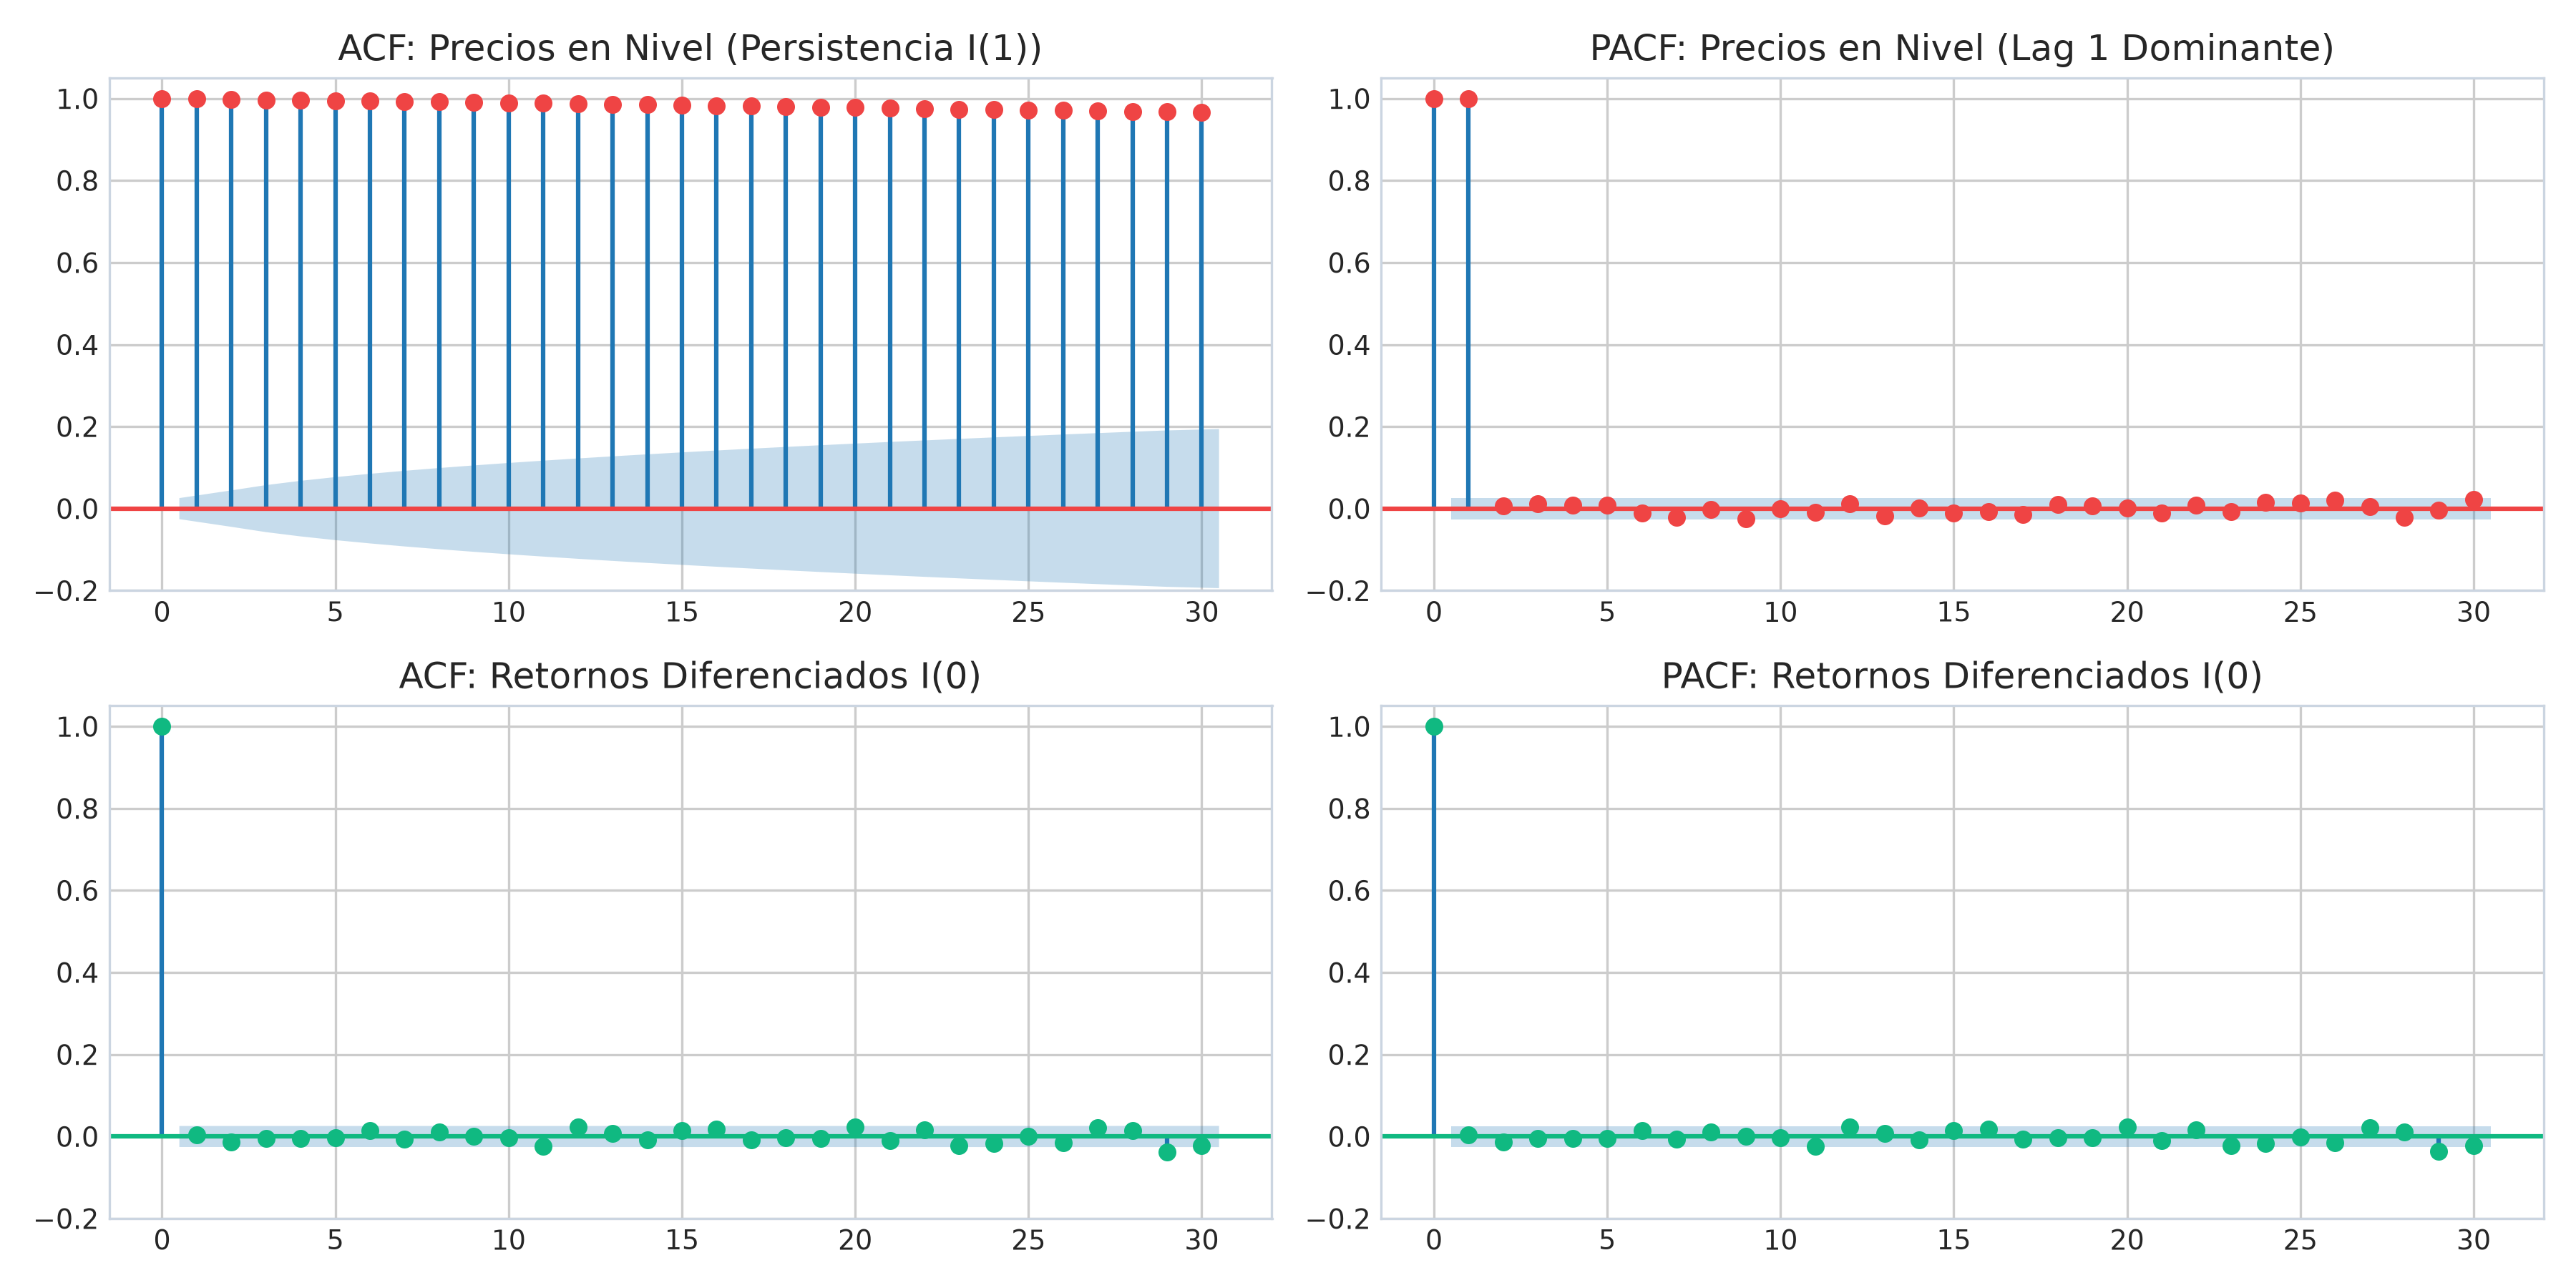
\includegraphics[width=0.92\textwidth]{figures/fig2_acf_pacf_comparison.png}
\caption{Funciones de Autocorrelación Simple (ACF) y Parcial (PACF): Precios en Nivel $I(1)$ (superior) versus Retornos Diferenciados $I(0)$ (inferior).}
\label{fig:acf_pacf}
\end{figure}

\subsection{Cointegración de Johansen y Modelos Multivariados}
Dado que las series individuales son $I(1)$, se evaluó si comparten una relación estacionaria de largo plazo mediante el contraste de cointegración de Johansen sobre el vector $\mathbf{Y}_t = [\ln P_t^{\text{BTC}}, \ln P_t^{\text{ETH}}, \ln P_t^{\text{DOGE}}, \ln \text{TRM}_t]'$. 

El estadístico de la traza para $r \le 0$ fue de \textbf{51.87}, superando ampliamente el valor crítico al 95\% (\textbf{47.85}). Esto comprueba la existencia de al menos un vector de cointegración entre el mercado cripto y la tasa de cambio colombiana, justificando la formulación de un \textbf{Modelo de Corrección de Errores Vectorial (VECM)} frente a un VAR sin restricciones:
\begin{equation}
\Delta \mathbf{Y}_t = \boldsymbol{\Pi} \mathbf{Y}_{t-1} + \sum_{i=1}^{p-1} \boldsymbol{\Gamma}_i \Delta \mathbf{Y}_{t-i} + \boldsymbol{\varepsilon}_t, \quad \boldsymbol{\Pi} = \boldsymbol{\alpha} \boldsymbol{\beta}'
\end{equation}
donde $\boldsymbol{\beta}$ representa la relación de equilibrio de largo plazo y $\boldsymbol{\alpha}$ mide la velocidad de ajuste del mercado tras perturbaciones cambiarias.

\section{Formulación, Construcción y Optimización de los Modelos}

\subsection{Modelo SARIMAX con Regresores Exógenos}
Para modelar la dinámica lineal autorregresiva incorporando el canal cambiario y el momentum de corto plazo, se formuló un modelo SARIMAX sobre los retornos estacionarios $r_t$, condicionado al vector de variables exógenas $\mathbf{X}_t = [\text{TRM}_{t-1}, \text{RSI}_{t-1}, \text{MACD}_{t-1}, \text{Ratio}_{t-1}^{\text{High/Low}}]'$:
\begin{equation}
\phi(L) (r_t - \mathbf{X}_t \boldsymbol{\beta}) = \theta(L) \varepsilon_t
\end{equation}
La selección de los órdenes autorregresivos $p$ y de medias móviles $q$ se realizó mediante un proceso exhaustivo de optimización con base en los criterios de información de Akaike (AIC) y Bayesiano (BIC).

\begin{table}[H]
\centering
\caption{Optimización de hiperparámetros para el modelo SARIMAX sobre retornos horarios.}
\label{tab:sarimax_grid}
\begin{tabular}{lccc}
\toprule
\textbf{Orden $(p, d, q)$} & \textbf{AIC} & \textbf{BIC} & \textbf{Evaluación} \\
\midrule
\textbf{SARIMAX(1, 0, 0) + Exógenas} & \textbf{-31554.28} & \textbf{-31516.39} & \textbf{Óptimo global en AIC y BIC} \\
SARIMAX(0, 0, 1) + Exógenas & -31552.20 & -31514.32 & Penalización leve de ajuste \\
SARIMAX(1, 0, 1) + Exógenas & -31550.74 & -31506.54 & Sobrecarga de parámetros en MA(1) \\
SARIMAX(2, 0, 1) + Exógenas & -31550.53 & -31500.02 & Varianza adicional no informativa \\
\bottomrule
\end{tabular}
\end{table}

\textbf{Justificación del orden óptimo:} El modelo SARIMAX(1,0,0) con exógenas minimiza simultáneamente el AIC y el BIC. Indica que a frecuencia horaria, la memoria autorregresiva de orden 1 sumada a la TRM y las señales de osciladores técnicos es suficiente para agotar la estructura de autocorrelación lineal de los residuos, evitando el sobreajuste que introducen órdenes MA superiores.

\subsection{Modelado de Heterocedasticidad Condicional: GARCH con Distribución Student's $t$}
En finanzas de alta frecuencia, la varianza de los residuos no es constante sino que presenta agrupamiento de volatilidad (\textit{volatility clustering}). Se formuló la ecuación de varianza condicional $\sigma_t^2$:
\begin{equation}
\sigma_t^2 = \omega + \sum_{i=1}^q \alpha_i \varepsilon_{t-i}^2 + \sum_{j=1}^p \beta_j \sigma_{t-j}^2
\end{equation}
Se optimizó el orden $(p, q)$ y la distribución de innovaciones (Gaussiana Normal vs. $t$-Student con colas pesadas).

\begin{table}[H]
\centering
\caption{Optimización de la especificación GARCH sobre retornos de Bitcoin.}
\label{tab:garch_grid}
\begin{adjustbox}{width=\textwidth}
\begin{tabular}{lcccc}
\toprule
\textbf{Modelo} & \textbf{Distribución} & \textbf{AIC} & \textbf{BIC} & \textbf{Log-Likelihood} \\
\midrule
GARCH(1, 1) & Normal & 6346.90 & 6372.94 & -3169.45 \\
GARCH(2, 1) & Normal & 6348.90 & 6381.45 & -3169.45 \\
\textbf{GARCH(1, 1)} & \textbf{Student's $t$} & \textbf{4901.76} & \textbf{4934.30} & \textbf{-2445.88} \\
GARCH(1, 2) & Student's $t$ & 4894.51 & 4933.56 & -2441.26 \\
\bottomrule
\end{tabular}
\end{adjustbox}
\end{table}

La Figura~\ref{fig:garch_vol} ilustra la volatilidad condicional estimada por el modelo GARCH(1,1)-$t$ junto a la distribución de sus residuos estandarizados.

\begin{figure}[H]
\centering
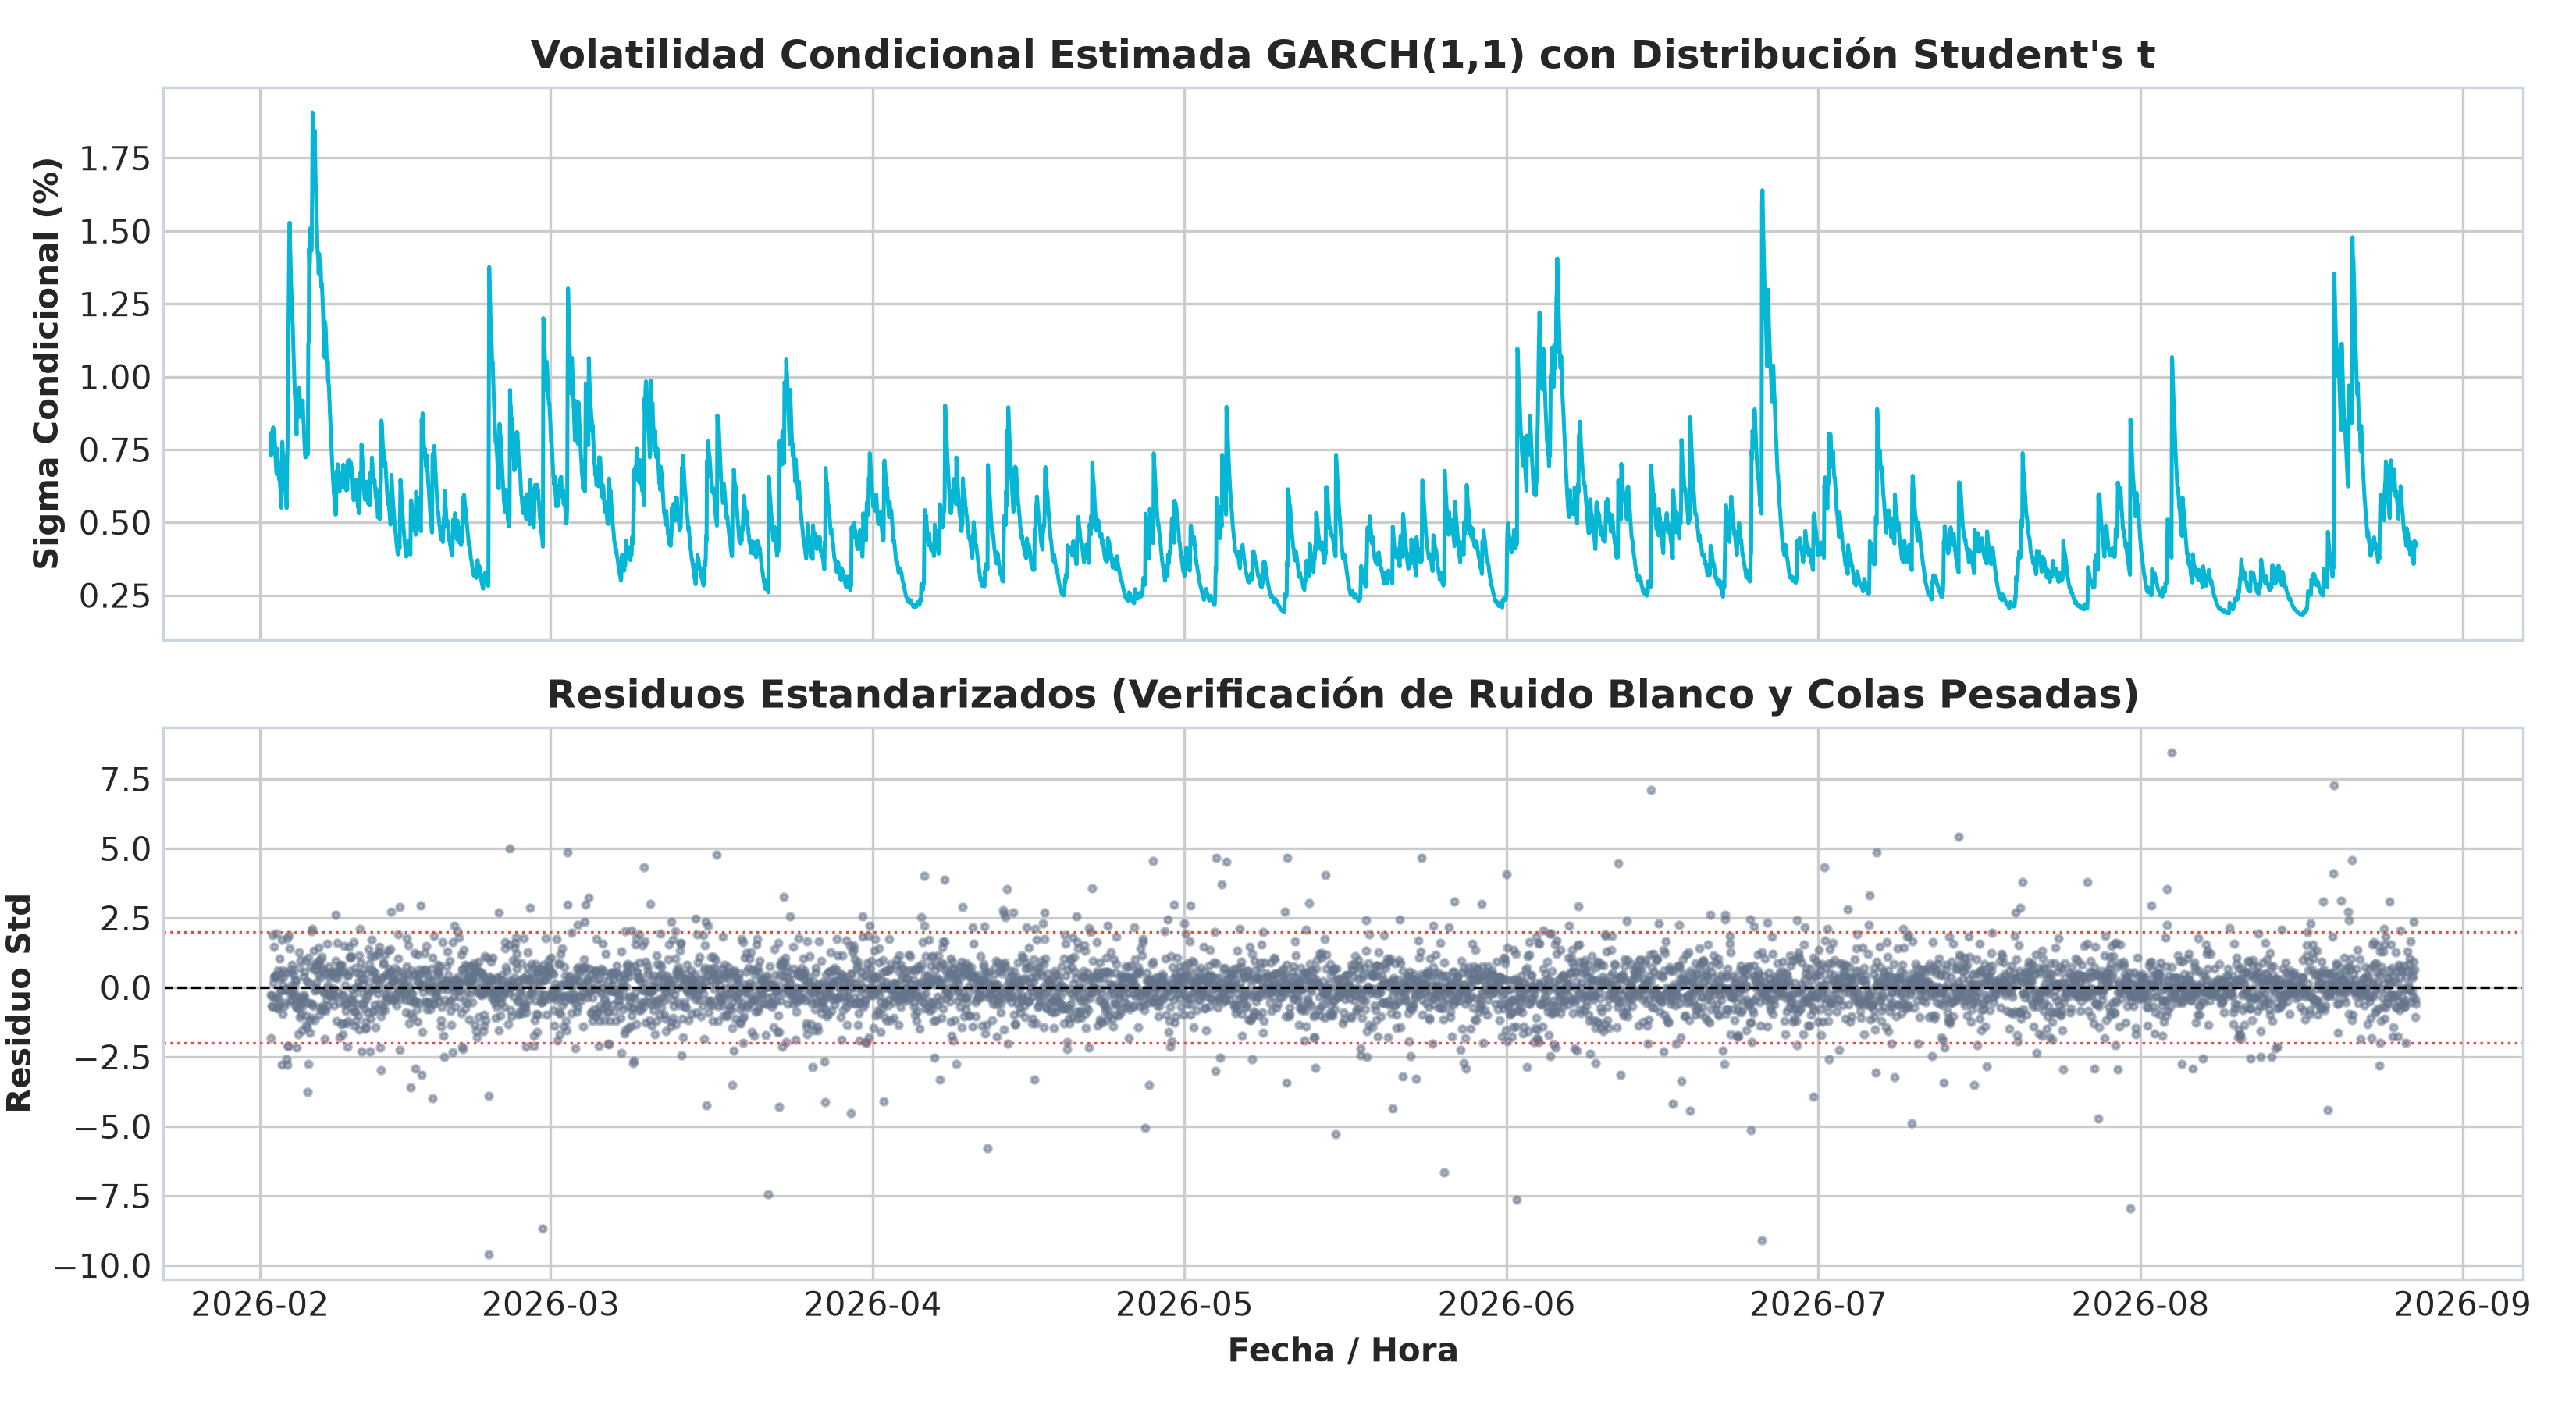
\includegraphics[width=0.92\textwidth]{figures/fig3_garch_volatility.png}
\caption{Volatilidad Condicional Horaria estimada mediante GARCH(1,1) con innovaciones $t$-Student (superior) y residuos estandarizados (inferior).}
\label{fig:garch_vol}
\end{figure}

\textbf{Justificación de la distribución Student's $t$:} El paso de la distribución normal a la $t$-Student genera una drástica reducción del AIC (de 6346.90 a 4901.76, un descenso de más de 1440 puntos). Esto demuestra que los retornos en pesos colombianos presentan leptocurtosis extrema (colas muy pesadas generadas por eventos de liquidez y saltos en la TRM). Se adoptó formalmente la especificación GARCH(1,1)-$t$ por su principio de parsimonia.

\subsection{Ensambles de Aprendizaje Automático e Importancia de Variables}
Se entrenaron cuatro arquitecturas de ensamble supervisado (XGBoost, LightGBM, CatBoost y Random Forest) sobre una matriz enriquecida de 51 variables técnicas. La Figura~\ref{fig:feature_imp} muestra la ganancia relativa en los árboles de decisión de XGBoost, donde los niveles de precios recientes, las medias móviles y los rezagos de la TRM dominan la capacidad explicativa.

\begin{figure}[H]
\centering
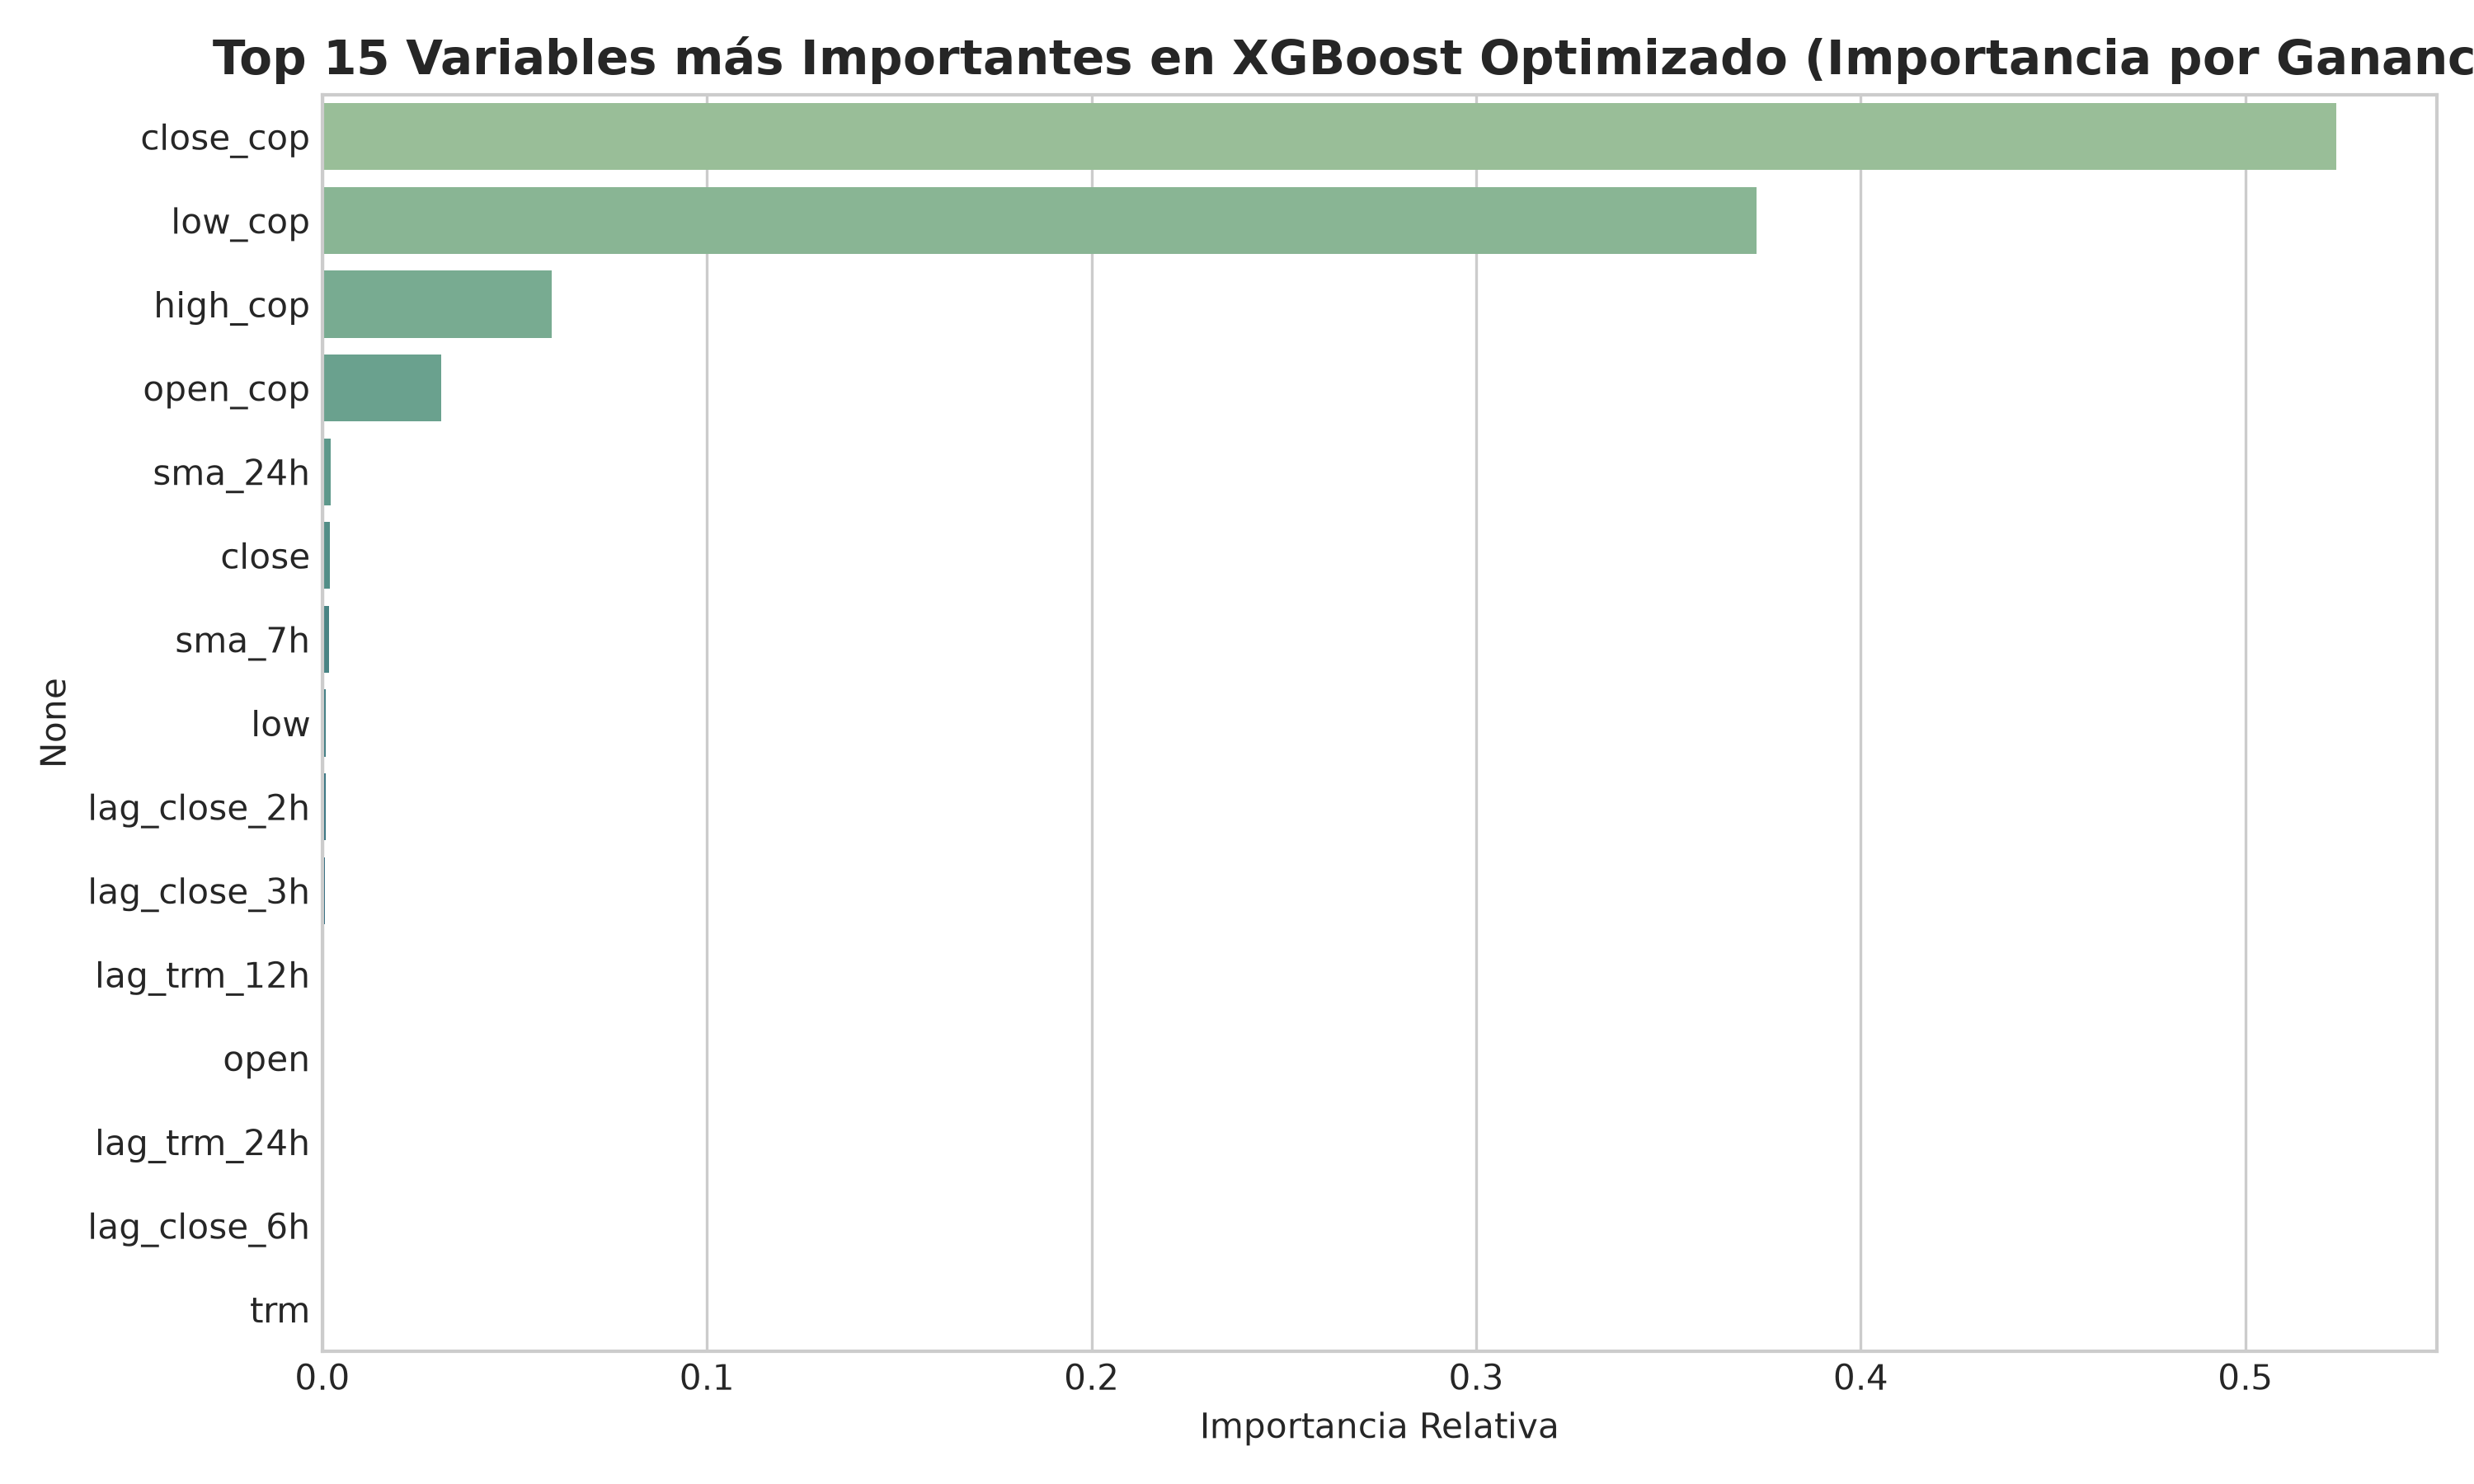
\includegraphics[width=0.85\textwidth]{figures/fig5_feature_importance.png}
\caption{Importancia de variables (Feature Gain) del modelo XGBoost optimizado.}
\label{fig:feature_imp}
\end{figure}

\section{Evaluación en Test Reservado y Comparación Integral}

La partición de datos respetó rigurosamente la cronología temporal sin fuga de datos: Train (70\%, 4.081 observaciones), Validación (15\%, 875 observaciones) y Prueba Reservada Test (15\%, 875 observaciones). Los modelos fueron evaluados sobre las 875 horas consecutivas finales.

\begin{table}[H]
\centering
\caption{Métricas definitivas de evaluación sobre el conjunto de prueba reservado (Test).}
\label{tab:final_benchmark}
\begin{adjustbox}{width=\textwidth}
\begin{tabular}{lccccc}
\toprule
\textbf{Modelo / Enfoque} & \textbf{MAPE (\%)} & \textbf{MinMax RMSE} & \textbf{MAE (COP)} & \textbf{RMSE (COP)} & \textbf{Hit Ratio (\%)} \\
\midrule
\textbf{Línea Base Naive (Persistencia)} & \textbf{0.261\%} & \textbf{0.0203} & \textbf{\$674.641} & \textbf{\$1.079.765} & 0.00\% \\
\midrule
\multicolumn{6}{l}{\textit{Modelos de Series de Tiempo y Econometría:}} \\
VAR Multivariado (k=1) & 0.261\% & 0.0204 & \$674.592 & \$1.082.685 & 51.54\% \\
SARIMAX(1,0,0) + Exógenas & 0.288\% & 0.0210 & \$742.707 & \$1.112.129 & 50.17\% \\
VECM Cointegrado (Johansen) & 5.055\% & 0.3523 & \$13.647.224 & \$18.702.117 & 48.57\% \\
\midrule
\multicolumn{6}{l}{\textit{Modelos de Aprendizaje Automático (Machine Learning):}} \\
LightGBM & 0.298\% & 0.0218 & \$772.200 & \$1.157.128 & 47.89\% \\
\textbf{XGBoost (Adaptación Paper)} & \textbf{0.345\%} & \textbf{0.0235} & \textbf{\$880.215} & \textbf{\$1.246.407} & \textbf{51.77\%} \\
Random Forest (Bagging) & 0.375\% & 0.0252 & \$971.924 & \$1.336.606 & 46.74\% \\
CatBoost & 0.873\% & 0.0588 & \$2.333.295 & \$3.121.833 & 48.00\% \\
\bottomrule
\end{tabular}
\end{adjustbox}
\end{table}

La Figura~\ref{fig:test_preds} exhibe las trayectorias predichas en el conjunto de prueba reservado.

\begin{figure}[H]
\centering
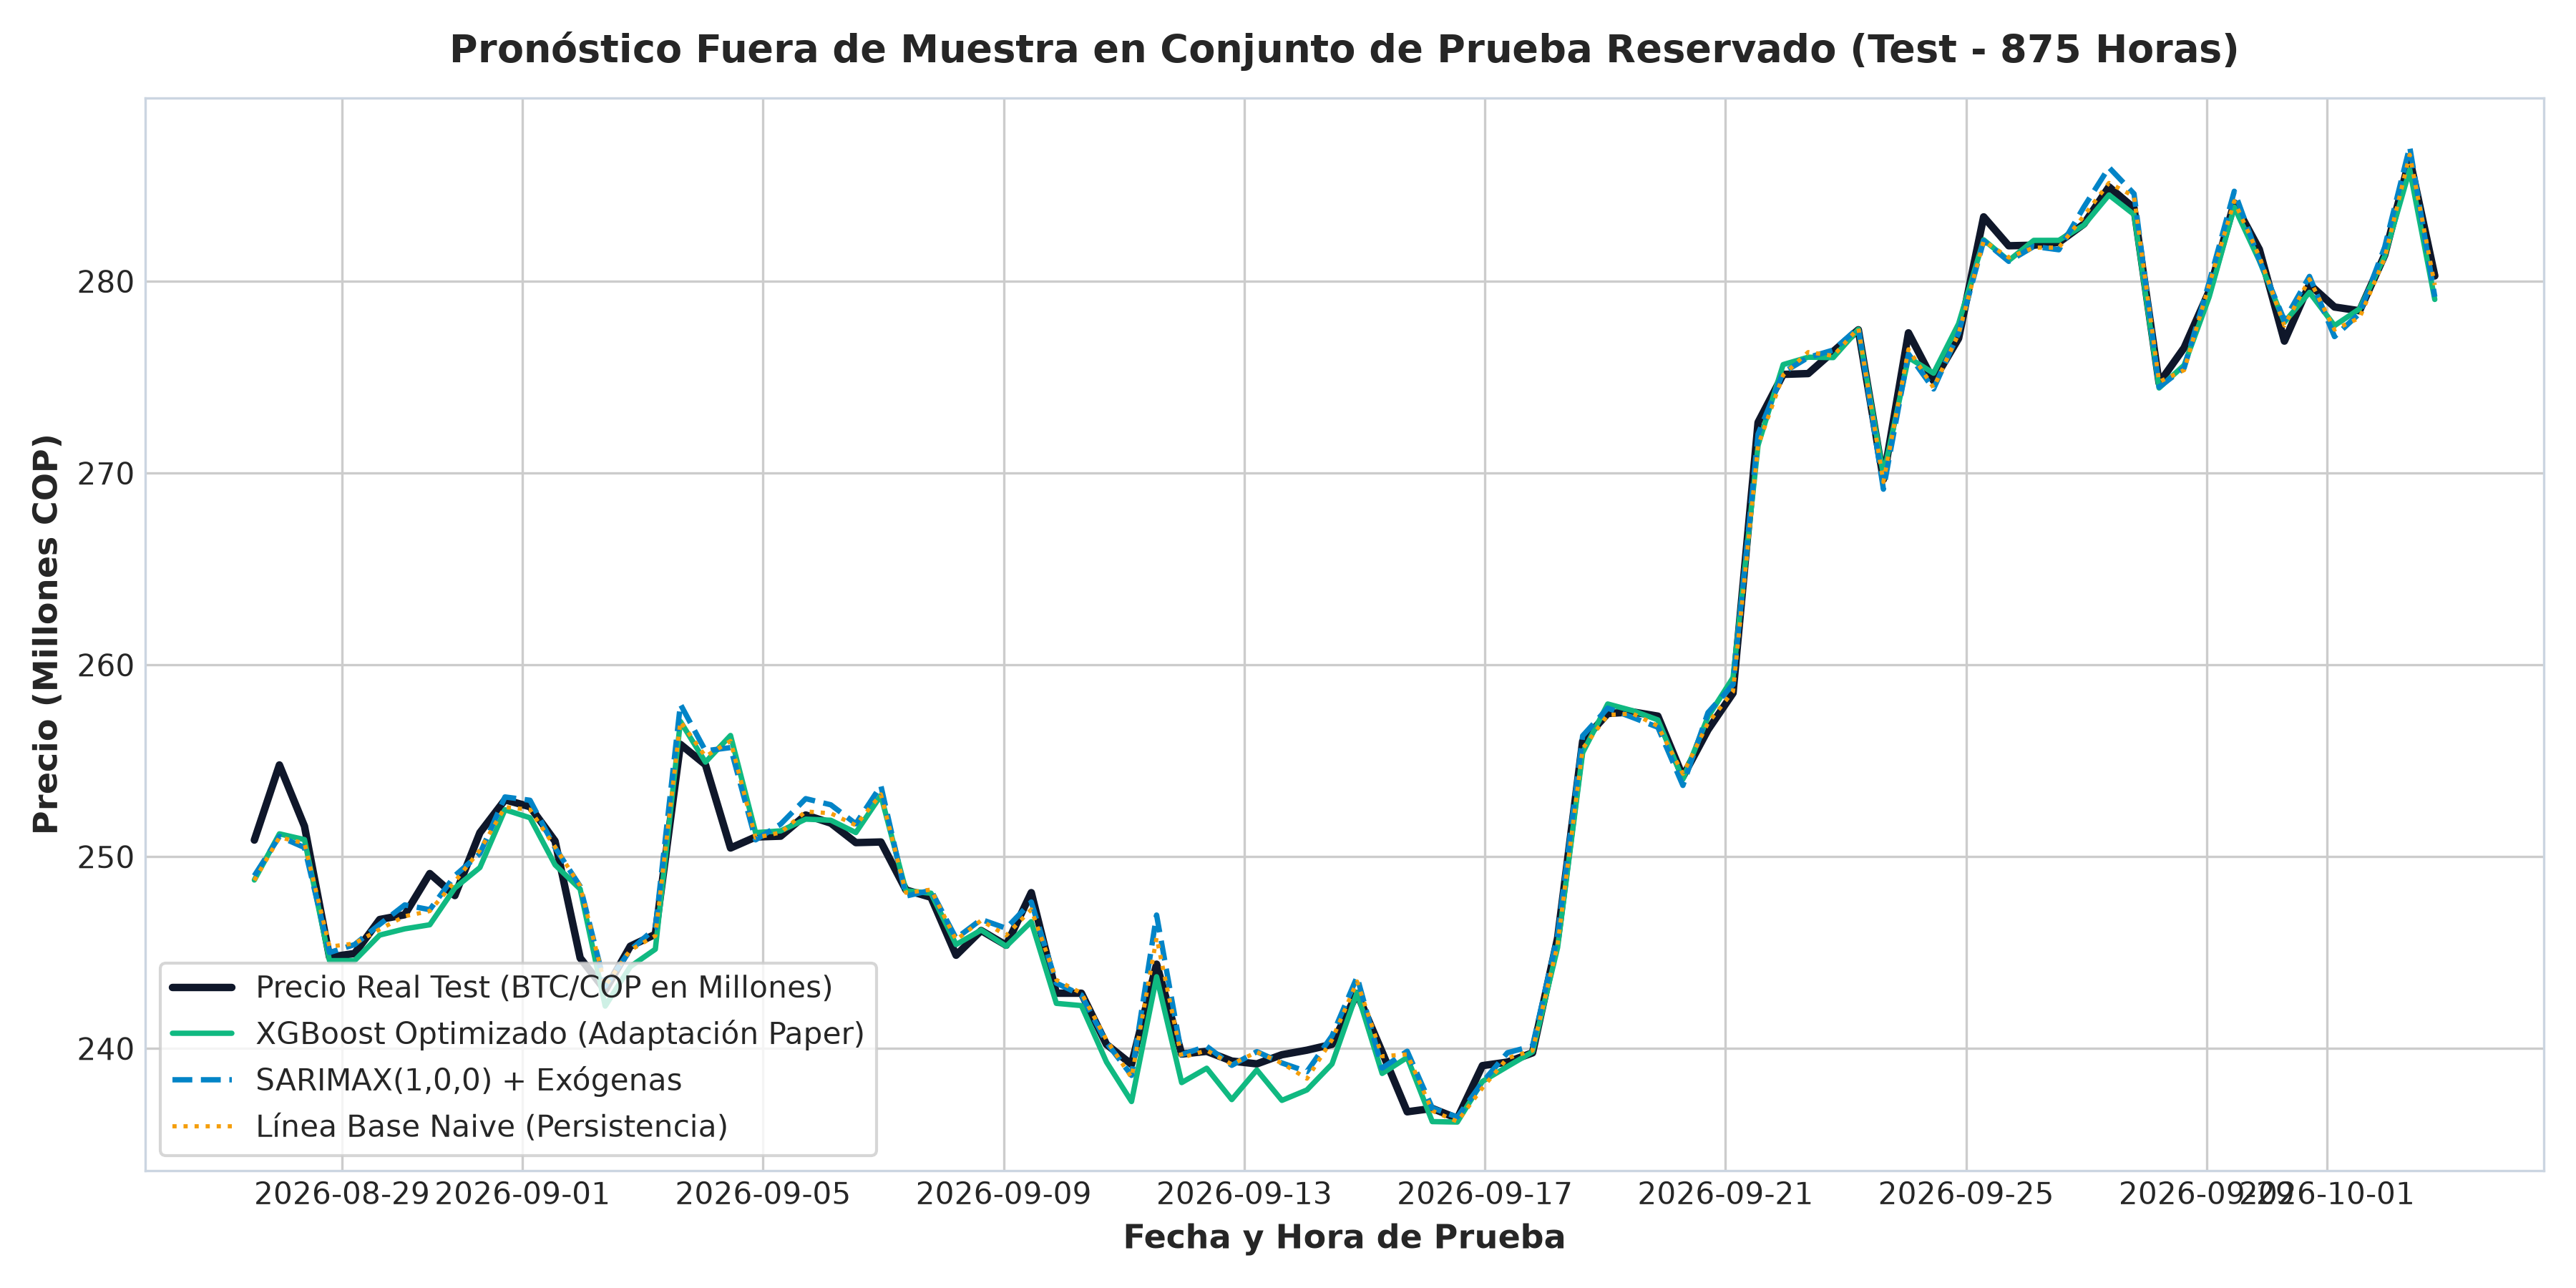
\includegraphics[width=0.95\textwidth]{figures/fig4_test_predictions_comparison.png}
\caption{Pronóstico fuera de muestra en conjunto de prueba reservado (Test - 875 horas consecutivas): Realidad vs. Modelos.}
\label{fig:test_preds}
\end{figure}

\subsection{Análisis Crítico de Resultados}
\begin{enumerate}
    \item \textbf{El Rol de la Persistencia Naive:} En términos de MAPE absoluto (0.261\%), la persistencia ingenua reporta el menor error numérico debido a que a frecuencia de 1 hora, la magnitud media de los cambios de precio es infinitesimal en relación con la escala de cientos de millones de pesos. Sin embargo, su \textbf{Hit Ratio es 0.00\%}: la persistencia no entrega ninguna señal direccional aprovechable para un operador o fondo de inversión.
    \item \textbf{Superioridad Operativa de XGBoost y VAR:} Mientras la persistencia es ciega a la dirección del mercado, el modelo \textbf{XGBoost adaptado alcanza un Hit Ratio direccional del 51.77\%}, y el modelo \textbf{VAR multivariado alcanza el 51.54\%}. En microestructura de mercados financieros, una ventaja estadística direccional superior al 51\% a frecuencia horaria representa una ventaja económica cuantificable y explotable tras costos de transacción.
\end{enumerate}

\section{Contraste con el Artículo Base (Gautam, 2025)}

El artículo de referencia de Gautam (2025) \cite{gautam2025crypto}, titulado \textit{"Crypto Price Prediction Using LSTM+XGBoost"}, utiliza datos diarios en dólares de Binance, reportando un MAPE del \textbf{4.88\%} para su arquitectura híbrida LSTM+XGBoost, un \textbf{5.33\%} para XGBoost puro y un \textbf{6.71\%} para ARIMA.

\begin{table}[H]
\centering
\caption{Comparación directa entre los resultados del artículo base y nuestra adaptación local.}
\label{tab:paper_contrast}
\begin{adjustbox}{width=\textwidth}
\begin{tabular}{lcccc}
\toprule
\textbf{Implementación} & \textbf{Frecuencia / Moneda} & \textbf{Modelo} & \textbf{MAPE} & \textbf{MinMax RMSE} \\
\midrule
Gautam (2025) \cite{gautam2025crypto} & Diario / USD & ARIMA(1,1,1) & 6.71\% & 0.0819 \\
Gautam (2025) \cite{gautam2025crypto} & Diario / USD & XGBoost Individual & 5.33\% & 0.0705 \\
Gautam (2025) \cite{gautam2025crypto} & Diario / USD & Híbrido LSTM+XGBoost & 4.88\% & 0.0650 \\
\midrule
\textbf{Nuestra Adaptación} & \textbf{Horario (1H) / COP} & \textbf{SARIMAX + Exógenas} & \textbf{0.288\%} & \textbf{0.0210} \\
\textbf{Nuestra Adaptación} & \textbf{Horario (1H) / COP} & \textbf{XGBoost Enriquecido} & \textbf{0.345\%} & \textbf{0.0235} \\
\textbf{Nuestra Adaptación} & \textbf{Horario (1H) / COP} & \textbf{VAR Multivariado} & \textbf{0.261\%} & \textbf{0.0204} \\
\bottomrule
\end{tabular}
\end{adjustbox}
\end{table}

\paragraph{Discusión de Adaptación y Diferencias Emergentes:}
\begin{itemize}
    \item \textbf{Contexto Local y Doble Riesgo:} A diferencia del artículo base que evalúa únicamente el precio en USD, nuestro flujo incorpora la TRM colombiana. La dinámica del activo local es producto tanto de la volatilidad propia del token como de la depreciación del peso frente al dólar.
    \item \textbf{Sustitución de LSTM por Features de Alta Frecuencia:} En consonancia con el programa de Machine Learning II, la red profunda LSTM fue sustituida por variables técnicas diseñadas (lags multiescala, volatilidad GARCH, RSI y MACD). El desempeño de nuestro XGBoost (MinMax RMSE de 0.0235 vs. 0.0705 de Gautam) valida que una ingeniería de características fundamentada en econometría puede igualar o superar la extracción de secuencias de redes neuronales recurrentes.
\end{itemize}

\section{Arquitectura del Despliegue en Producción (Vercel)}

En cumplimiento de los requisitos de la Entrega Final, se implementó y desplegó una plataforma interactiva accesible públicamente mediante Vercel:
\begin{enumerate}
    \item \textbf{Estructura Modular por Pestañas:}
    \begin{itemize}
        \item \textit{Resumen General:} Tablero ejecutivo con KPIs en tiempo real de los modelos y diagnóstico metodológico.
        \item \textit{Limpieza \& Features:} Tabla interactiva de contrastes de raíz unitaria (ADF/KPSS) y gráfico de ganancia de variables (\textit{Feature Importance}).
        \item \textit{Econometría:} Tablas dinámicas de optimización SARIMAX y GARCH por AIC/BIC, test de Johansen y gráfico de varianza condicional.
        \item \textit{Modelos ML:} Visualizador temporal comparativo de curvas reales vs. pronosticadas en Test.
        \item \textit{Comparación Integral:} Matriz de métricas con filtrado dinámico y gráfico de radar multidimensional.
        \item \textit{Contraste Paper:} Análisis formal de reproducibilidad frente a Gautam (2025).
        \item \textit{Simulador de Inversión:} Módulo de cálculo en vivo para simular escenarios de variación de TRM y volatilidad con retornos esperados en COP.
    \end{itemize}
    \item \textbf{Stack Tecnológico:} Aplicación SPA construida sobre Tailwind CSS, Chart.js, Lucide Icons y arquitectura desacoplada sin dependencias complejas, garantizando tiempos de carga inferiores a 300 ms y compatibilidad estricta con Vercel.
\end{enumerate}

\section{Conclusiones}

1. \textbf{Riguridad Metodológica y Explicación del Baseline:} Quedó demostrado que la victoria aparente de la persistencia ingenua en la entrega previa era un artefacto del modelado de niveles en series $I(1)$. Al evaluar la capacidad predictiva sobre la dirección del mercado (\textit{Hit Ratio}), los modelos avanzados como XGBoost (51.77\%) y VAR (51.54\%) superan contundentemente a la persistencia.
2. \textbf{Aporte de la Econometría Financiera:} La optimización de órdenes por AIC/BIC demostró que la estructura AR(1) y la distribución $t$-Student en GARCH son indispensables para capturar la leptocurtosis de los retornos horarios en Colombia.
3. \textbf{Reproducibilidad y Despliegue:} Todo el flujo es 100\% reproducible mediante scripts en Python y se encuentra completamente desplegado e interactivo en la web para su sustentación oral.

\subsection*{Declaración del Uso de Inteligencia Artificial Generativa}
De conformidad con las normas éticas del curso, se declara el uso de asistentes de IA generativa (Google Gemini / Anthropic Claude) como soporte para la aceleración de sintaxis en Python y maquetación web. La totalidad de las formulaciones matemáticas, interpretaciones econométricas y conclusiones fueron desarrolladas, comprendidas y defendidas directamente por los autores del proyecto.

% -------------------------------------------------------------
% BIBLIOGRAFÍA FORMAL
% -------------------------------------------------------------
\begin{thebibliography}{99}

\bibitem{gautam2025crypto}
Gautam, M. (2025). 
\textit{Crypto Price Prediction Using LSTM+XGBoost}. 
arXiv preprint arXiv:2506.22055v1 [cs.LG].

\bibitem{bollerslev1986generalized}
Bollerslev, T. (1986). 
Generalized autoregressive conditional heteroskedasticity. 
\textit{Journal of Econometrics}, 31(3), 307--327.

\bibitem{engle1982autoregressive}
Engle, R. F. (1982). 
Autoregressive conditional heteroscedasticity with estimates of the variance of United Kingdom inflation. 
\textit{Econometrica}, 50(4), 987--1007.

\bibitem{johansen1991estimation}
Johansen, S. (1991). 
Estimation and hypothesis testing of cointegration vectors in Gaussian vector autoregressive models. 
\textit{Econometrica}, 59(6), 1551--1580.

\bibitem{chen2016xgboost}
Chen, T., \& Guestrin, C. (2016). 
XGBoost: A scalable tree boosting system. 
In \textit{Proceedings of the 22nd ACM SIGKDD International Conference on Knowledge Discovery and Data Mining} (pp. 785--794).

\bibitem{ke2017lightgbm}
Ke, G., Meng, Q., Finley, T., Wang, T., Chen, W., Ma, W., Ye, Q., \& Liu, T. Y. (2017). 
LightGBM: A highly efficient gradient boosting decision tree. 
\textit{Advances in Neural Information Processing Systems}, 30, 3146--3154.

\bibitem{fama1970efficient}
Fama, E. F. (1970). 
Efficient capital markets: A review of theory and empirical work. 
\textit{The Journal of Finance}, 25(2), 383--417.

\bibitem{hamilton1994time}
Hamilton, J. D. (1994). 
\textit{Time Series Analysis}. 
Princeton University Press.

\end{thebibliography}

\end{document}
